% !TEX root = 15cvpr.tex
\section{Experiments}

\subsection{Experimental Setup}
For a given dataset, we employ the Multiscale Combinatorial Grouping System \cite{arbelaez2014multiscale} 

In particular, we extract a 4296 dimensional feature vector for each image by concatenating appearance feature and topic distribution. The 4296 dimensional feature vector includes: the second to last layer of convolutional neural network\cite{simonyan2014very} pre-trained on ImageNet \cite{russakovsky2014imagenet}, as the appearance feature, and topic distribution which learned from pLSA \cite{hofmann1999probabilistic}, as topic distribution.

As an illustration, Figure shows the inter-label correlation matrix illustrating the inter-dependency between 33 categories on the SiftFlow dataset. The brighter the block is, the stronger co-occurrence between labels exists. The dark blocks indicate the concepts pairs without correlation on the dataset.
Among these pairs of the different concepts, we find that the concept pair of television and sofa have strong correlation.


\subsection{Comparison with State of the Art}
In this section, we compare our approach with the existing state of the art weakly supervised semantic segmentation methods as well as fully supervised semantic segmentation algorithms on two real-world datasets: PASCAL VOC 2007 \cite{pascal-voc-2007} and SIFT-flow \cite{liu2011nonparametric}.

\begin{table*}[htp] \small
\begin{center}
\begin{tabular}{l|l|c| p{1mm} p{1mm} p{1mm} p{1mm} p{1mm} p{1mm} p{1mm} p{1mm} p{1mm} p{1mm} p{1mm} p{1mm} p{1mm} p{1mm} p{1mm} p{1mm} p{1mm} p{1mm} p{1mm} p{1mm} p{1mm} p{1mm}}

& Methods & \rotatebox{90}{average} & \rotatebox{90}{background} & \rotatebox{90}{aeroplane} & \rotatebox{90}{bicycle} & \rotatebox{90}{bird} & \rotatebox{90}{boat} & \rotatebox{90}{bottle} & \rotatebox{90}{bus} & \rotatebox{90}{car} & \rotatebox{90}{cat} & \rotatebox{90}{chair} & \rotatebox{90}{cow} & \rotatebox{90}{diningtable} & \rotatebox{90}{dog} & \rotatebox{90}{horse} & \rotatebox{90}{motorbike} & \rotatebox{90}{person} & \rotatebox{90}{pottedplant} & \rotatebox{90}{sheep} & \rotatebox{90}{sofa} & \rotatebox{90}{train} & \rotatebox{90}{tv/monitor} \\
\hline
 & Brookes & 9 & 78 & 6 & 0 & 0 & 0 & 0 & 9 & 5 & 10 & 1 & 2 & 11 & 0 & 6 & 6 & 29 & 2 & 2 & 0 & 11 & 0 \\
 Fully & INRIA \cite{ferrari2008groups} & 24 & 3 & 1 & 45 & 34 & 16 & 20 & 0 & 68 & 58 & 11 & 0 & 44 & 8 & 1 & 2 & 59 & 37 & 0 & 6 & 19 & 63 \\
 Supervised& MPI \cite{lampert2008beyond} & 28 & 3 & 30 & 31 & 10  & 41 & 7 & 8 & 73 & 56 & 37 & 11 & 19 & 2 & 15 & 24 & 67 & 26 & 9 & 3 & 5 & 55\\
 & TKK \cite{VISUAL2008voc} & 30 & 23 &19 & 21 & 5 & 16 & 3 & 1 & 78 & 1 & 3 & 1 & 23 & 69 & 44 & 42 & 0 & 65 & 30 & 35 & 89 & 71 \\
 & UoCTTI \cite{felzenszwalb2008discriminatively} & 21 & 3 & 24 & 53 & 0 & 2 & 16 & 49 & 33 & 1 & 6 & 10 & 0 & 0 & 3 & 21 & 60 & 11 & 0 & 26 & 72 & 58 \\
\hline
Weakly & Zhang \etal \cite{zhang2013sparse} & 24 & $-$ & 48 & 20 & 26 & 25 & 3 & 7 & 23 & 13 & 38 & 19 & 15 & 39 & 17 & 18 & 25 & 47 & 9 & 41 & 17 & 33 \\
Supervised& Ours & 27 & 66 & 26 & 15 & 61 & 12 & 15 & 51 & 30 & 38 & 6 & 29 & 19 & 25 & 29 & 26 & 19 & 12 & 18 & 4 & 28 & 28 \\
\end{tabular}
\caption{Quantitative analysis of VOC2007 results \cite{pascal-voc-2007}, intersection vs. union measure, define as $\frac{TP}{TP + FN + FP}$, in comparison with state-of-the-art methods. The results of fully supervised methods are taken from \cite{pascal-voc-2007}. }
\label{tab:ExpVOC_test}
\end{center}
\vskip -0.1in
\end{table*}

\textbf{PASCAL VOC 2007}
This dataset was used for the PASCAL Visual Object Category segmentation contest 2007. It is especially challenging for the presence of background clutter, illumination effect and occlusions. It contains 5011 training images, and 4952 test images. Within the training set, for a subset of 422 images which are suitable for evaluation of the segmentation task, the object in these images are marked at pixel level, while the objects in the other images only have the bounding boxes indicating the location of the object and rough boundaries. And there are 20 foreground and 1 background classes in this dataset used for the task of classification, detection, and segmentation.


\textbf{SIFT-flow} The SIFT Flow dataset\cite{liu2011nonparametric} is derived from the LabelMe subset and contains 2688 images of resolution 256x256 pixels, accompanied with a hand labeled segmentation of 33 unique semantic categories. This dataset has been widely adopted for semantic segmentation and it is also very challenging for the reason that there are large number of classes in the dataset and $4.43$ classes per image. Besides, the frequency of classes is distributed with a pow-low. For fair comparison, we use standard dataset split (2488 images for training and 200 images for testing) provided by \cite{liu2011nonparametric}.

\textbf{Quantitative and Qualitative Results} Comparisons of our performances against other methods (both fully supervised and weakly supervised) are given in Tables \ref{tab:ExpVOC_test} and \ref{tab:ExpSIFTflow_Test}. The results on the VOC2007 dataset show that our approach outperforms the other state-of-the-art weakly supervised methods, demonstrating that the image-level annotation are more efficiently utilized by our method. In the meantime, the results conducted by our framework is comparable with the fully supervised method even though we use much less supervised information than these methods. Similar results are obtain on SIFT-flow dataset, which is more challenging than the previous one. Figures \ref{fig:VOC-2007} and \ref{fig:SIFT-flow} show the success and failure cases of three dataset respectively.

\begin{table}[!h]
\begin{center}
\begin{tabular}{|c|c|c|c|}
\hline
Methods & Supervision & Per-Class (\%) \\
\hline
Liu \etal \cite{liu2011nonparametric} & full & 24 \\
Tighe \etal \cite{tighe2010superparsing} & full & 29.4 \\
Tighe \etal \cite{Tighe2013Finding} & full & 39.2 \\
\hline
Vezhnevets \etal \cite{vezhnevets2011weakly} & weak & 14 \\
Vezhnevets \etal \cite{vezhnevets2012weakly} & weak & 21 \\
Zhang \etal \cite{zhang2013sparse} & weak & 26 \\
Zhang \etal \cite{zhang2013probabilistic} & weak & 27.7 \\
Xu \etal \cite{xu2014tell} & weak & 27.9 \\
Ours & weak & 30.2 \\
\hline
\end{tabular}
\end{center}
%\vspace{-3mm}
\caption{Quantitative results on the SIFT-flow dataset \cite{liu2011nonparametric}, average per-class recall measure, defined as $\frac{TP}{TP+FN}$, in comparison with state-of-the-art methods. }
\label{tab:ExpSIFTflow_Test}
\end{table}

\subsection{Performance under the Noisy Condition}
To verify both robustness and effectiveness of our method to noisy annotation condition, we try to add some noise to the initial image-level labels for SiftFlow dataset. More concretely, for a certain image in the dataset, each image-level label might be missing or replaced by other incorrect labels. Suppose the probability of missing label is $p_{missing}$, and the probability of labeling category $i$ instead of category $j$ is $p_{ij}$ which is based on the empirical evidence from the collaborative image tagging system, \eg Flickr. We fix the probability $p_{ij}$, and set different values of $p_{missing}$ to obtain a set of noisy labeled datasets. Then we perform a controlled test on these noisy dataset. As shown in Table \ref{tab:ExpNoise}, our approach is robust under the noisy condition. 



\begin{table}[!h]
\begin{center}
\begin{tabular}{|c|c|c|c|c|}
\hline
Experiment Setting & exp1 & exp2 & exp3 & exp4 \\
\hline
Noisy Image (\%) & 23.2 & 33.8 & 53.4 & 77.8 \\
\hline
Noisy Labels per Image & 1.4 & 1.5 & 1.8 & 2.4 \\
\hline
Per-Class accuracy (\%) & 29.8 & 29.1 & 28.1 & 22.3 \\
\hline
\end{tabular}
\end{center}
%\vspace{-3mm}
\caption{Quantitative results  }
\label{tab:ExpNoise}
\end{table}


\begin{figure}[h]
\begin{center}
    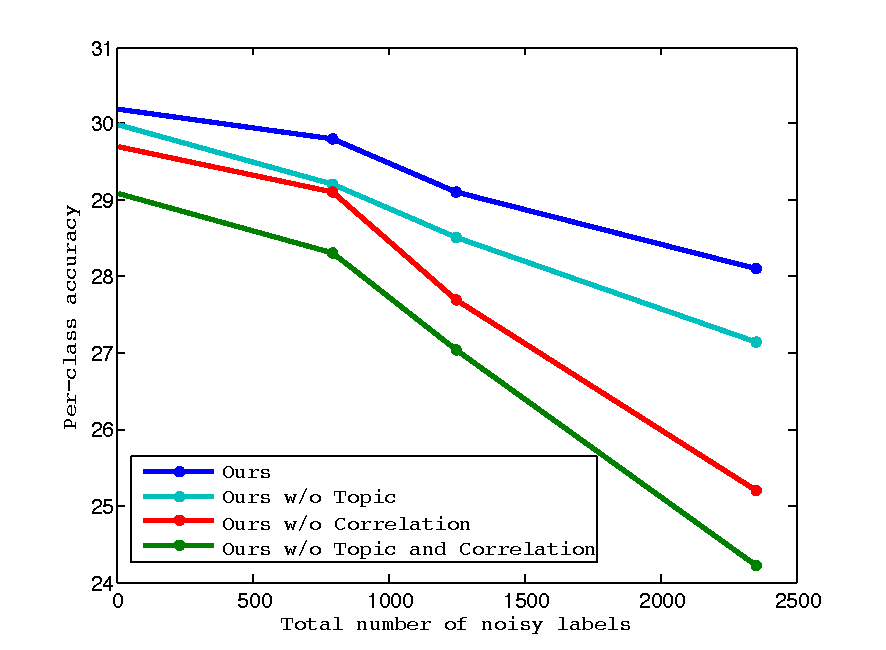
\includegraphics[width=1\linewidth]{fig_noisylabel.pdf}
\end{center}
    \caption{}
\label{fig:noisyexp}
\end{figure}


\begin{figure*}
\begin{center}
	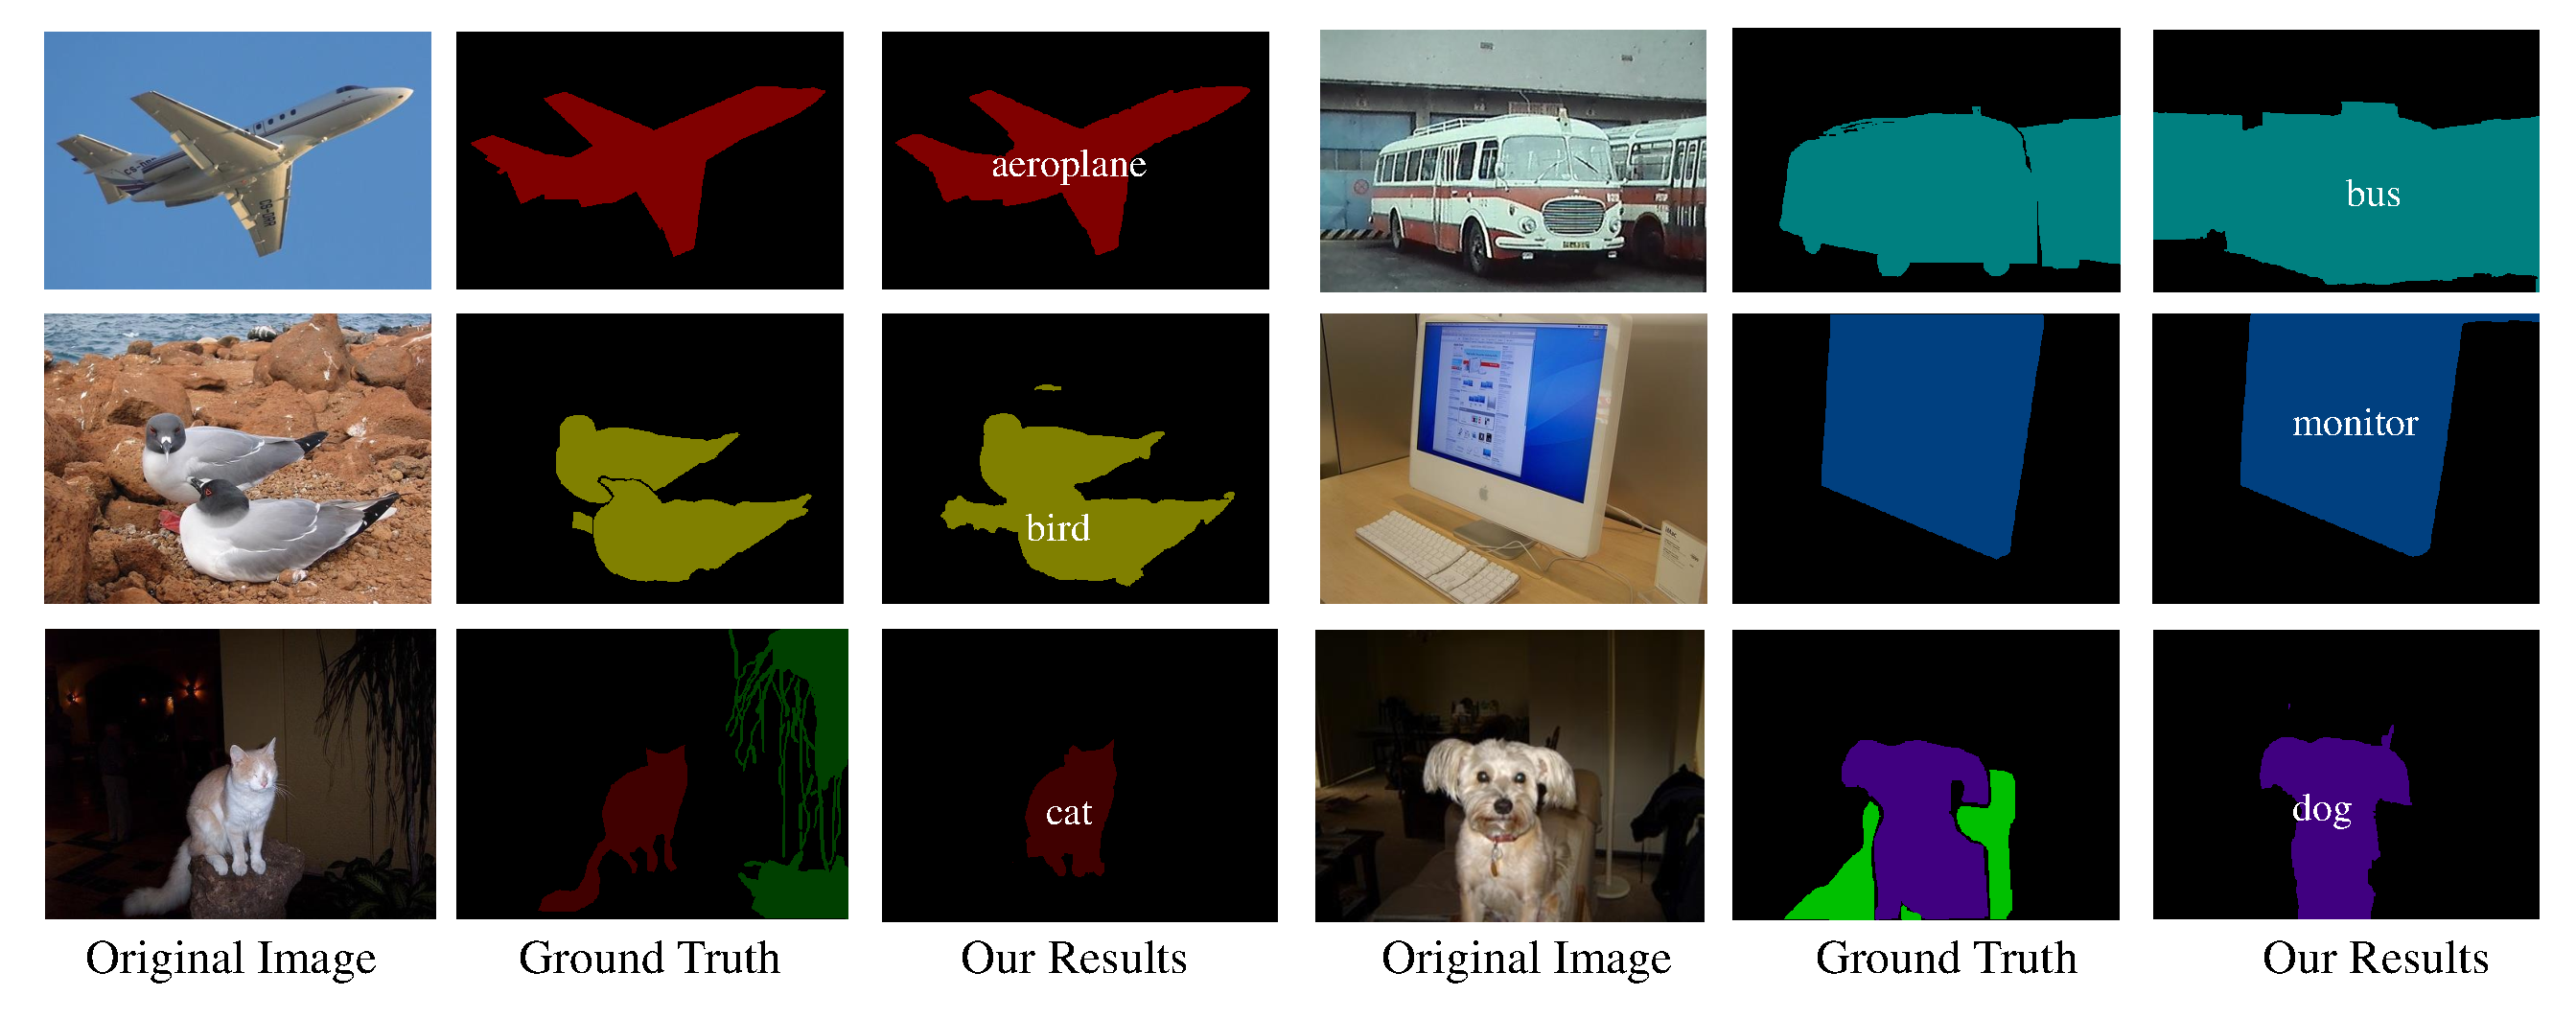
\includegraphics[width=1\linewidth]{Fig_VOC.pdf}
\end{center}
   \caption{Qualitative results on the VOC-2007 data set. Successful segmentations (top 2 rows) and failure cases (bottom).}
\label{fig:VOC-2007}
\end{figure*}

\begin{figure*}
\begin{center}
	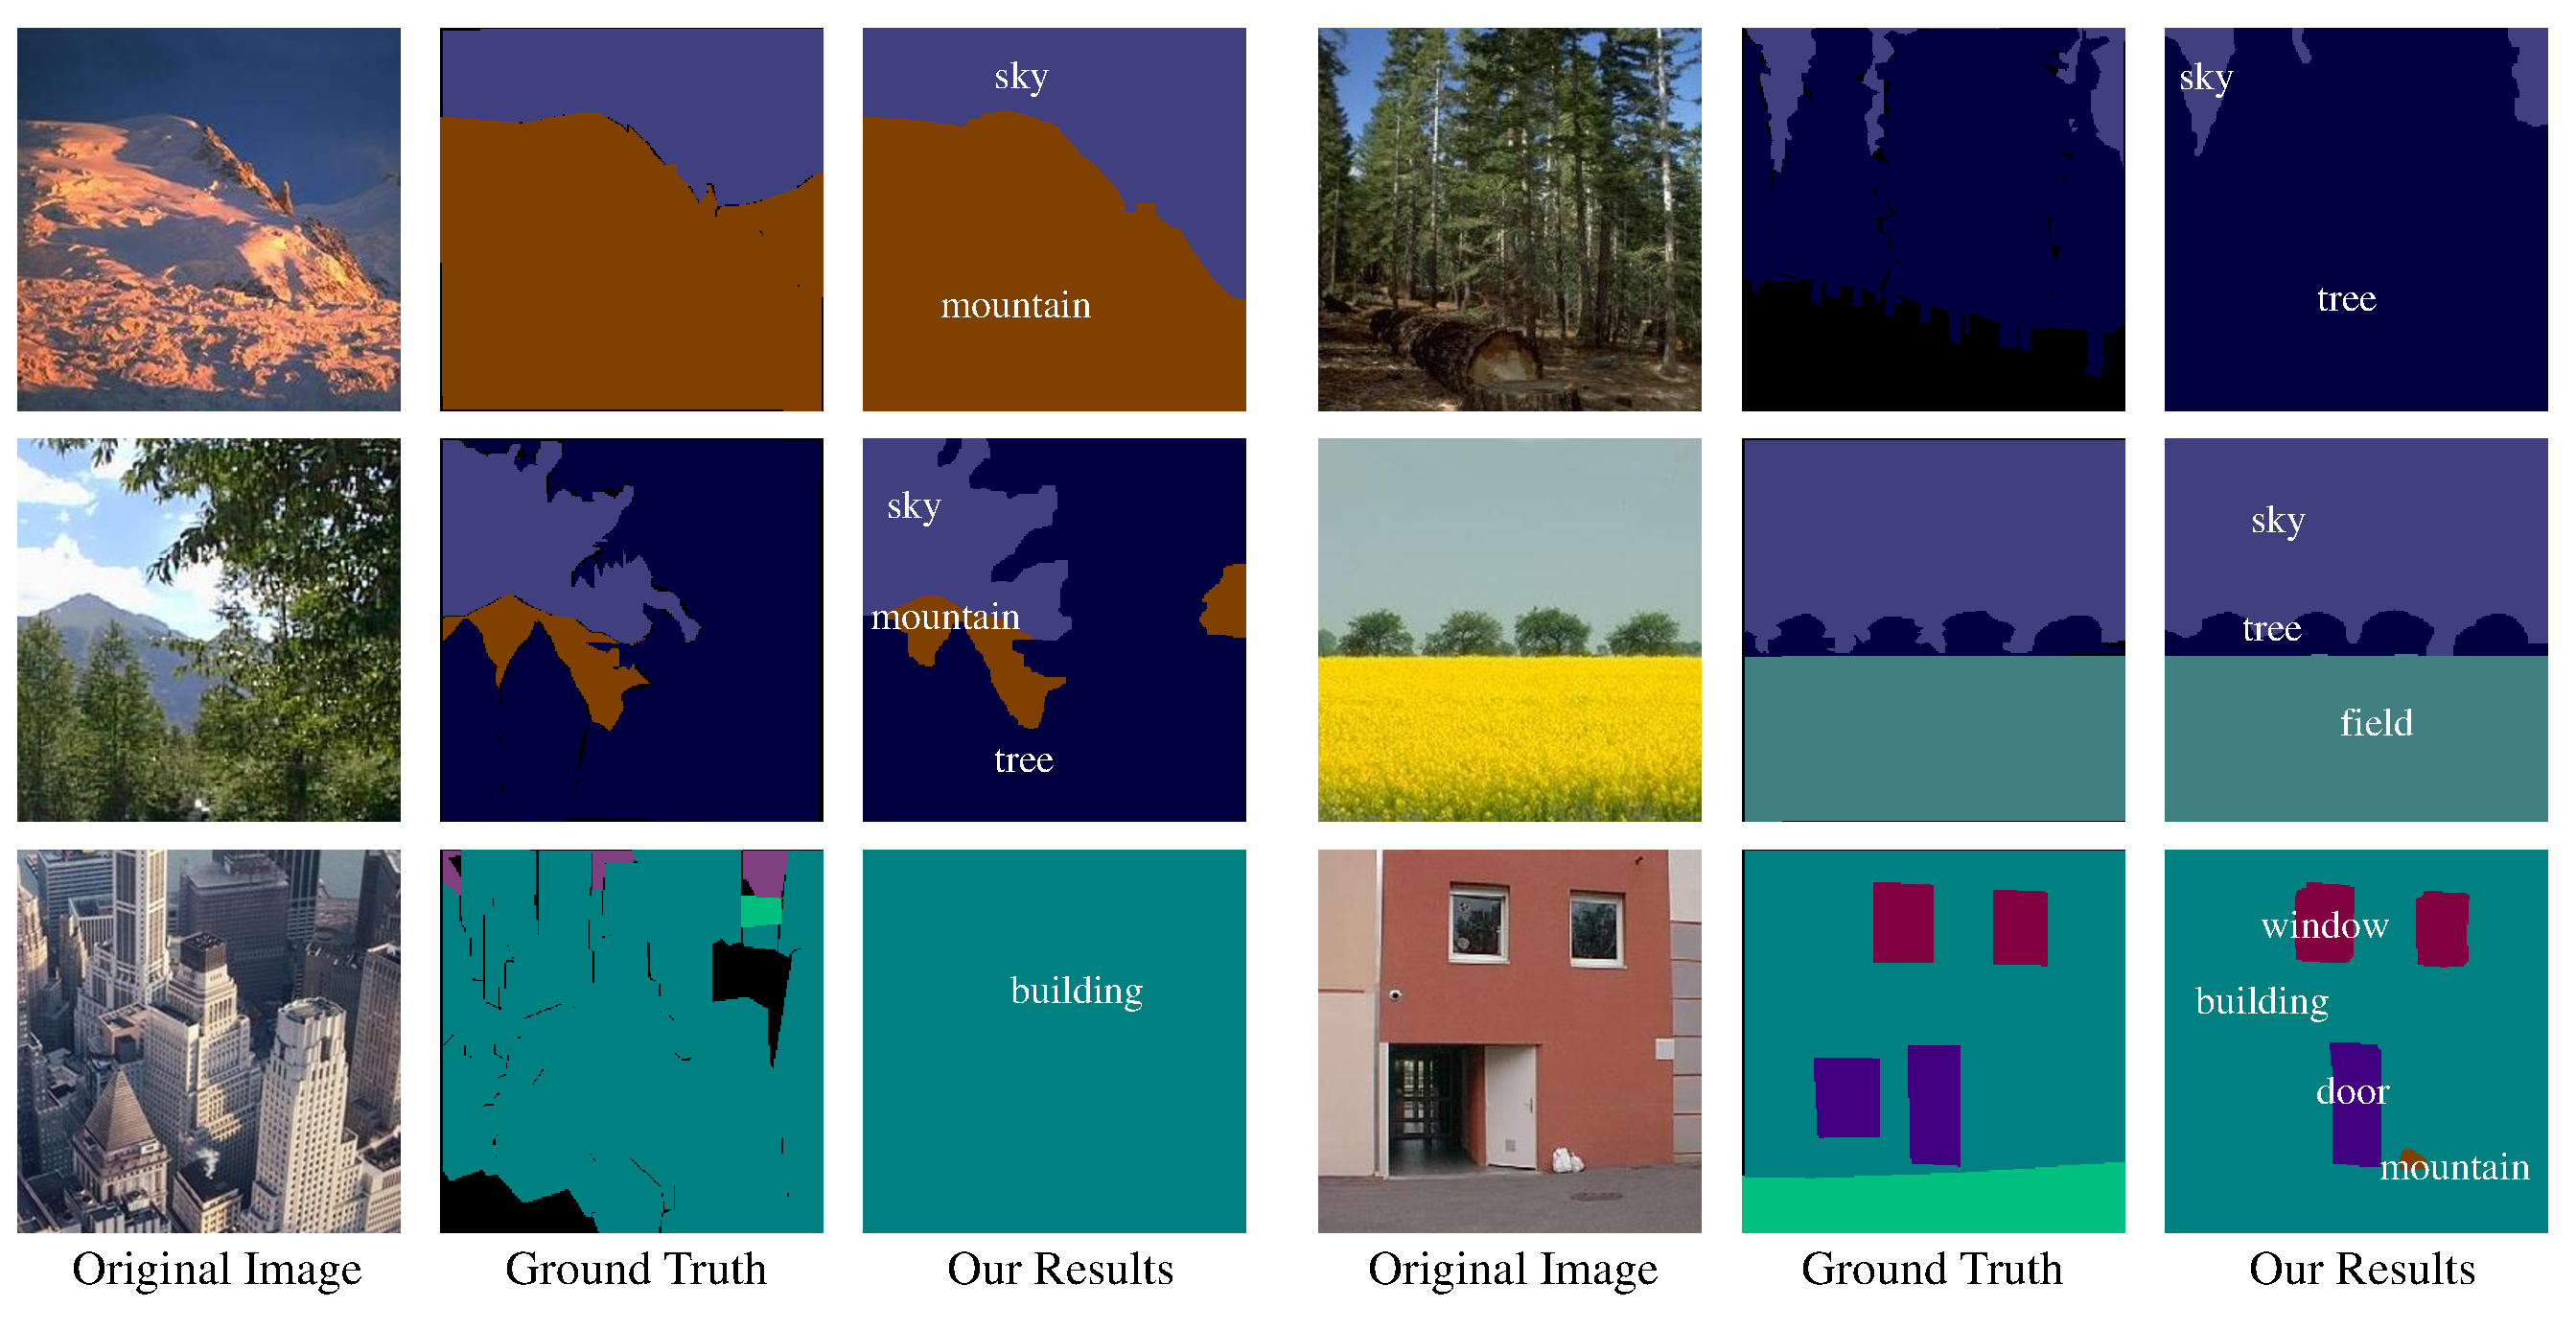
\includegraphics[width=1\linewidth]{Fig_SIFTflow.pdf}
\end{center}
   \caption{Qualitative results on the SIFT-flow data set. Successful segmentations (top 2 rows) and failure cases (bottom).}
\label{fig:SIFT-flow}
\end{figure*}


